\documentclass[12pt]{article}
\usepackage[spanish]{babel}
%\usepackage[utf8]{inputenc} 
\usepackage{makeidx}
\usepackage{multirow}
\usepackage{multicol}
\usepackage[dvipsnames,svgnames,table]{xcolor}
\usepackage{graphicx}
\usepackage{epstopdf}
\usepackage{ulem}
\usepackage[hidelinks]{hyperref} 
\usepackage{amsmath}
\usepackage{amssymb}
\usepackage[paperwidth=595pt,paperheight=841pt,top=56pt,right=86pt,bottom=84pt,left=71pt]{geometry}
\usepackage{setspace}
\title{Titulo}
\onehalfspacing


\makeatletter
	\newenvironment{indentation}[3]%
	{\par\setlength{\parindent}{#3}
	\setlength{\leftmargin}{#1}       \setlength{\rightmargin}{#2}%
	\advance\linewidth -\leftmargin       \advance\linewidth -\rightmargin%
	\advance\@totalleftmargin\leftmargin  \@setpar{{\@@par}}%
	\parshape 1\@totalleftmargin \linewidth\ignorespaces}{\par}%
\makeatother 



\begin{document}
\textbf{{\large UNIVERSIDAD DE M\'{A}LAGA}}

\textbf{ESCUELA T\'{E}CNICA SUPERIOR DE INGENIER\'{I}A INFORM\'{A}TICA}
\textbf {INGENIERA T\'{E}CNDCA EN INFORM\'{O}TICA IE GESTI\'{A}N}

\textbf{ALGORITMOS PARA MANIPULACI\'{O}N DE IMPLICACIONES EN AN\'{A}LISIS DE
CONCEPTOS FORMALES}

\textbf{Realizado por}
\\
\textbf{ADORACI\'{O}N M\textordfeminine{} CALDER\'{O}N RIVAS}

\textbf{Dirigido por}
\\
\textbf{\'{A}NGEL MORA BONLLLA}

Departamento
\\
\textbf{MATEM\'{A}TICA APLICADA}

\textbf{M\'{A}LAGA, (mes y a\~{n}o)}

\newpage

{\large \textbf{UNIVERSIDAD DE M\'{A}LAGA}
\\
\textbf{ESCUELA T\'{E}CNICA SUPERIOR DE INGENIER\'{I}A INFORM\'{A}TICA}}

INGENIER\'{I}A T\'{E}CNICA EN INFORM\'{A}TICA DE GESTI\'{O}N

Reunido el tribunal examinador en el d\'{\i}a de la fecha, constituido por:


\leavevmode \\
Presidente/a D\textordmasculine{}/D\textordfeminine{}.
\_\_\_\_\_\_\_\_\_\_\_\_\_\_\_\_\_\_\_\_\_\_\_\_\_\_\_\_\_\_\_\_\_\_\_\_\_\_\_\_


\leavevmode \\
Secretario/a D\textordmasculine{}/D\textordfeminine{}.
\_\_\_\_\_\_\_\_\_\_\_\_\_\_\_\_\_\_\_\_\_\_\_\_\_\_\_\_\_\_\_\_\_\_\_\_\_\_\_\_


\leavevmode \\
Vocal D\textordmasculine{}/D\textordfeminine{}.
\_\_\_\_\_\_\_\_\_\_\_\_\_\_\_\_\_\_\_\_\_\_\_\_\_\_\_\_\_\_\_\_\_\_\_\_\_\_\_\_\_\_\_\_\_\_


\leavevmode \\
para juzgar el proyecto Fin de Carrera titulado:

\_\_\_\_\_\_\_\_\_\_\_\_\_\_\_\_\_\_\_\_\_\_\_\_\_\_\_\_\_\_\_\_\_\_\_\_\_\_\_\_\_\_\_\_\_\_\_\_\_\_\_\_\_\_\_\_


\leavevmode \\
realizado por D\textordmasculine{}/D\textordfeminine{}
\_\_\_\_\_\_\_\_\_\_\_\_\_\_\_\_\_\_\_\_\_\_\_\_\_\_\_\_\_\_\_\_\_\_\_\_\_\_\_\_\_


\leavevmode \\
tutorizado por D\textordmasculine{}/D\textordfeminine{}.
\_\_\_\_\_\_\_\_\_\_\_\_\_\_\_\_\_\_\_\_\_\_\_\_\_\_\_\_\_\_\_\_\_\_\_\_\_\_ ,



y, en su casa, dirigido acad\'{e}micomente por


D\textordmasculine{}/D\textordfeminine{}.\_\_\_\_\_\_\_\_\_\_\_\_\_\_\_\_\_\_\_\_\_\_\_\_\_\_\_\_\_\_\_\_\_\_\_\_\_\_\_\_\_\_\_\_\_\_\_\_\_\_\_\_


\_\_\_\_\_\_\_\_\_\_\_\_\_\_\_\_\_\_\_\_\_\_\_\_\_\_\_\_\_\_\_\_\_\_\_\_\_\_\_\_\_\_\_\_\_\_\_\_\_\_\_\_\_\_\_\_\_



ACORD\'{O} POR \_\_\_\_\_\_\_\_\_\_\_\_\_\_\_\_\_\_\_\_\_ OTORGAR LA
CALIFICACI\'{O}N

DE
\_\_\_\_\_\_\_\_\_\_\_\_\_\_\_\_\_\_\_\_\_\_\_\_\_\_\_\_\_\_\_\_\_\_\_\_\_\_\_\_\_\_

Y PARA QUE CONSTE, SE EXTIENDE FIRMADA POR LOS COMPARECIENTES DEL TRIBUNAL, LA
PRESENTE DILIGENCIA.

M\'{a}laga a \_\_\_\_ de\_\_\_\_\_\_\_\_\_\_\_\_\_\_ del 200\_

\newpage

\tableofcontents
\newpage

\section{INTRODUCCI\'{O}N}
	\subsection{Historia}
	

		El An\'{a}lisis de Conceptos Formales (FCA) constituye una herramienta formal
		para el analisis de datos que permite la extracci\'{o}n de conocimiento  a
		partir de un conjunto de objetos y las propiedades que cumplen dichos objetos.
		
		La teor\'{\i}a en su forma actual se remonta al grupo de investigaci\'{o}n
		dirigido por Rudolf Darmstadt Wille, Bernhard Ganter y Peter Burmeister, donde se
		origin\'{o} el an\'{a}lisis de conceptos formales en la d\'{e}cada de 1980. La
		base matem\'{a}tica, sin embargo, ya se hab\'{\i}a creado por Garrett Birkhoff en
		la d\'{e}cada de los a\~{n}os 30 como parte de la teor\'{\i}a general de
		ret\'{\i}culos. Antes del trabajo del grupo de Darmstadt, ya extst\'{\i}an
		enfoques similares de varios grupos franceses, y sus fundamentos filos\'{o}ficos
		apuntan principalmente a Charles S. Peirce y el pedagogo Hartmut von Hentig.
		
		En su art\'{i}culo 
		\href{http://books.google.de/books?hl=de&lr=&id=gwpq0acO3kgC&oi=fnd&pg=PA314&dq=Wille+Restructuring+Lattice+Theory&ots=zYmNQeCJKb&sig=TyDygU5lU_91iJWIuJbNi2or6Ls#v=onepage&q=Wille Restructuring Lattice Theory&f=false}{"Reestructuraci\'{o}n de la Teor\'{i}a de Ret\'{i}culos"}
		(de 1982, con el que se inicia el FCA como disciplina matem\'{a}tica) Rudolf Wille parte de un descontento con la 
		teor\'{i}a de ret\'{i}culos en particular y con las matem\'{a}ticas puras en general: 
		
		La producci\'{o}n de resultados te\'{o}ricos - a menudo alcanzados por medio de "elaboradas 
		gimnasias mentales" - eran impresionantes, pero las conexiones entre dominios vecinos, o
		incluso entre partes de una misma teor\'{i}a se estaban debilitando.
		La reestructuraci\'{o}n de la teor\'{i}a de ret\'{i}culos es un intento de revitalizar las 
		conexiones entre dominios mediante la reinterpretaci\'{o}n de la teor\'{i}a de la manera m\'{a}s
		concreta posible, con el fin de propiciar una mejor comunicaci\'{o}n entre los te\'{o}ricos de 
		ret\'{i}culos y los usuarios potenciales de dicha teor\'{i}a. Este objetivo se remonta a Hartmut 
		von Hentig, quien en 1972 pidi\'{o} una reestructuraci\'{o}n de las ciencias con el fin de
		conseguir una mejor enseñanza y de hacer a la ciencia m\'{a}s asequible, tanto con el fin de 
		conocerla mejor como para poder criticarla de una forma m\'{a}s cercana (es decir, sin necesidad
		de un conocimiento especializado).
		
		El FCA corrige el punto de partida de la teor\'{i}a reticular en el desarrollo de la l\'{o}gica formal en 
		el siglo XIX, donde un concepto, como predicado unario, se hab\'{i}a reducido a su extensi\'{o}n. El 
		objetivo fue trabajar con una visi\'{o}n de los conceptos menos abstracta, haciendo uso tambi\'{e}n de la 
		intensi\'{o}n, una orientaci\'{o}n que proven\'{i}a de la lingü\'{i}stica y de la l\'{o}gica conceptual cl\'{a}sica.
		
		FCA tiene como objetivo aclarar los conceptos siguiendo la m\'{a}xima de Charles S. Peirce de desplegar 
		las propiedades observables y elementales de los objetos. En su filosof\'{i}a tard\'{i}a, Peirce supone que el 
		pensamiento l\'{o}gico tiene como objetivo percibir la realidad, por medio de la triada: concepto, 
		juicio y conclusi\'{o}n. En este sentido, Wille dice: 
		
		\textit{El objetivo y el significado del FCA como teor\'{i}a matem\'{a}tica sobre conceptos y sus jerarqu\'{i}as es 
		apoyar la comunicaci\'{o}n racional entre seres humanos mediante el desarrollo matem\'{a}tico de 
		estructuras conceptuales apropiadas que se puedan manipular con la l\'{o}gica.}
		
	\subsection{Contextos y conceptos}
		
		El FCA tiene como entrada una tabla con la relaci\'{o}n entre un conjunto de objetos (o conceptos) y 
		un conjunto de propiedades (atributos).  Esta entrada es lo que se  denomina \textbf{contexto 
		formal} y la relaci\'{o}n que se define en dicha tabla determina qu\`{e} objetos cumplen qu\`{e} propiedades.
		
		Un concepto formal se define como un par formado por  un conjunto de objetos (\textbf{extensi\'{o}n}) 
		y un conjunto de atributos (\textbf{intensi\'{o}n}) de forma que la extensi\'{o}n est\'{a} formada
		por todos los objetos que comparten los atributos dados y la intensi\'{o}n por los atributos 
		compartidos por los objetos dados.
		
		Por lo que, un \textbf{contexto formal} se puede definir como una tripleta \textit{K=(O,A,P)}, 
		donde \textit{O} es un conjunto de objetos, \textit{A} es un conjunto de atributos y \textit{P} 
		una relaci\'{o}n binaria, $P \subseteq O \times A$, que muestra qu\'{e} objeto posee qu\'{e} 
		atributo. Formalmente, se puede considerar como un grafo bipartito que refleje las relaciones 
		entre los conjuntos \textit{O} y \textit{A}, o tambi\'{e}n como una una tabla con los objetos 
		ocupando las filas de la tabla, los atributos en las columnas, y de forma que un valor booleano
		en la celda \textit{(x,y)} significa que el objeto \textit{x} tiene el atributo \textit{y}.\\
		
		\begin{figure}
			\begin{center}
				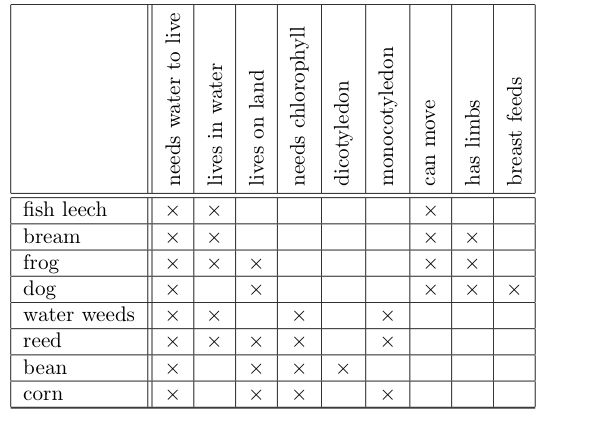
\includegraphics[scale=.5]{Figura1.png}
			\end{center}
			\caption{Contexto Formal}\label{Figura1}
		\end{figure}
		
	\subsection{Implicaciones y reglas de asociaci\'{o}n con FCA}
	
		Una vez formalizados matem\'{a}ticamente los conceptos, puede resultar relativamente sencillo trasladar 
		las relaciones l\'{o}gicas que encontramos entre atributos... aunque debemos tener en cuenta que las 
		relaciones l\'{o}gicas que se obtengan son aquellas que vengan confirmadas por nuestro contexto, 
		que podr\'{i}a representar un conocimiento concreto en un instante de tiempo, pero que podr\'{i}a 
		variar al añadir un mayor n\'{u}mero de objetos o atributos. Por ejemplo, que en el ejemplo 
		siguiente podamos decir que "ser animal de jungla "implica" ser mam\'{i}fero" se debe a que todos 
		los objetos que verifican la propiedad "ser animal de jungla" verifican "ser mam\'{i}fero", pero 
		en el momento que introduzcamos un objeto nuevo que sea de la jungla (por ejemplo, un manglar) y 
		no sea mam\'{i}fero, esa implicaci\'{o}n deja de ser cierta. Por supuesto, podemos trabajar con
		 varios atributos simult\'{a}neamente.
		
		Consecuentemente, en FCA podemos formalizarlo de la siguiente forma: dados \textit{A} y \textit{B}
		subconjuntos de atributos, diremos que se tiene la implicaci\'{o}n $A \to B$ si se verifica 
		$A′ subseteq B′$, es decir, todos los objetos que tienen cada atributo de \textit{A} tambi\'{e}n 
		tienen cada atributo de \textit{B} (observa que es coherente con la implicaci\'{o}n intuitiva que 
		dimos en el apartado anterior).
	
	Con esta definición, las implicaciones obedecen las reglas de Armstrong (reflexiva, aumentativa y transitiva) comunes en las dependencias funcionales que se dan entre los atributos de una base de datos:
	
	\[
		B \subseteq A A \to B, A \to B A \cup C \to B \cup C, X \to B, B \to C A\to C
	\]
		
	A partir de la definición de implicación y de las propiedades básicas que verifica, podemos definir un cálculo lógico que nos permitiría realizar sistemas de deducción completos sobre el contexto actual. En cierta forma, hemos pasado de tener un conocimiento por ejemplos a disponer de un conocimiento abstracto que introduce sistemas de razonamiento más elaborados en nuestro mundo, partiendo únicamente de las observaciones concretas que hemos realizado, es decir, hemos aprendido reglas generales a partir de ejemplos.
 
 	\subsection{Aplicaciones}
 	
 		Desde su introducción ha sido aplicado en campos tan variados como la minería de datos, minería de textos, gestión del conocimiento, web semántica, desarrollo de software, biología, etc.
 		
 		La doctora Karell Bertet, investigadora de la Universidad de La Rochelle con la que colabora el director del proyecto,  ha desarrollado una librería java, java-lattices, para la generación, representación y manipulación de los Conceptos Formales, etc. 
 		
 		Dicha librería implementa la generación de retículos. Se pueden generar:
 		\begin{itemize}
 			\item Un retículo dados los nodos y sus relaciones.
 			\item Álgebras booleanas de 2n elementos.
 			\item Retículos de permutaciones.
 			\item Retículos aleatorios de n nodos.
 			\item Retículos de Conceptos a partir de un contexto o de un conjunto de implicaciones.
 			\item Cálculo de Implicaciones y de bases de implicaciones.
 			\item Etc.
 		\end{itemize}
 		
\section{ANÁLISIS FORMAL DE CONCEPTOS}

	\subsection{¿Qué es FCA?}
	
	El Análisis de Conceptos Formales (FCA) es un método de análisis de datos con creciente popularidad en distintos ámbitos como puede ser la minería de datos, pre-procesamiento de datos o descubrimiento del conocimiento.
	
	FCA analiza los datos que describen  relaciones entre un conjunto de objetos y un conjunto de atributos y genera dos tipos de salida a partir de dichos datos. 
	
	El primer tipo es un \textbf{retículo de conceptos}. Un retículo de conceptos es un conjunto de conceptos formales ordenados jerárquicamente por una relación subconcepto-superconcepto.
	
	Los conceptos formales son agrupaciones que representan objetos, cosas, nociones como “organismos que viven en el agua”, “números divisibles por 3 y 4”, etc.
	
	Formalmente, se pueden definir los conceptos formales como pares \textit{(A, B)} donde $A \subseteq X$ es un conjunto de objetos y $B \subseteq Y$ es un conjunto de atributos,  tal que todos los elementos de \textit{A} tienen los atributos de \textit{B} y los elementos de \textit{B} son los atributos comunes a todos los objetos de \textit{A}.
	
	

				


\end{document}